\chapter{\diagTitle}\label{sec:diagonalization}



Given a linear transformation, it is highly desirable to write its matrix  with respect to a basis of eigenvectors.

\section{Diagonalizability}\index{Diagonalization}

Suppose we are lucky, and we have $L \colon V\to V$, and the ordered basis 
$B=(v_1, \ldots, v_n )$ is a set of %linearly independent 
eigenvectors for $L$, with eigenvalues $\lambda_1, \ldots, \lambda_n$.  Then:

\begin{eqnarray*}
L(v_1)&=&\lambda_1 v_1 \\
L(v_2)&=&\lambda_2 v_2 \\
&\vdots & \\
L(v_n)&=&\lambda_n v_n \\
\end{eqnarray*}
As a result, the matrix of $L$ in the basis of eigenvectors $B$ is diagonal:
\[
L\begin{pmatrix}
x^1\\
x^2\\
\vdots\\
x^n
\end{pmatrix}_B
=
\left(
\begin{pmatrix}
\lambda_1    \\
& \lambda_2 &  & \\
&  & \ddots &  \\
& & & \lambda_n
\end{pmatrix}
\begin{pmatrix}
x^1\\
x^2\\
\vdots\\
x^n
\end{pmatrix}
\right)_B
,
\]
where all entries off the diagonal are zero.

Suppose that \(V\) is any \(n\)-dimensional vector space. We call a linear transformation $L \colon V\mapsto V$ \emph{diagonalizable}\index{Diagonalizable} if there exists a collection of $n$ linearly independent eigenvectors for $L$.  In other words, $L$ is diagonalizable if there exists a basis for $V$ of eigenvectors for $L$.  

In a basis of eigenvectors, the matrix of a linear transformation is diagonal.  On the other hand, if an $n \times n$ matrix is diagonal, then the standard basis vectors $e_i$ must already be a set of $n$ linearly independent eigenvectors.  We have shown:

\begin{theorem}
Given an ordered basis $B$ for a vector space $V$ and a linear transformation $L \colon V\rightarrow V$, then the matrix for $L$ in the basis $B$ is diagonal if and only if $B$ consists of eigenvectors for $L$.
\end{theorem}

\Videoscriptlink{diagonalization_derivative.mp4}{Non-diagonalizable example}{scripts_diagonalization_derivative}

%\begin{center}\href{\webworkurl ReadingHomework20/2/}{Reading homework: problem 20.2}\end{center}
\Reading{Diagonalization}{1}

Typically, however, we do not begin a problem with a basis of eigenvectors, but rather have to compute these. Hence we need to know how to change from one basis to another:

\section{Change of Basis}\index{Change of basis}

Suppose we have two  ordered bases $S=(v_1, \ldots, v_n )$ and 
$S'=(v'_1, \ldots, v'_n )$ for a vector space $V$. (Here $v_i$ and $v'_i$ are {\it vectors}, not components of vectors in a basis!) 
Then we may write each $v'_k$ uniquely as 
\[
v'_k = \sum_i v_ip^i_k\, ,
\]
this is $v'_k$ as a linear combination of the~$v_i$. 
In  matrix notation
\[ 
\rowvec{v'_1 , v'_2 , \cdots , v'_n} = \rowvec{v_1 , v_2 , \cdots , v_n}
\begin{pmatrix}p^1_1&p^1_2&\cdots &p^1_n\\ p^2_1 & p^2_2 && \\[2mm]
                                              \mc\vdots &&&\mc\vdots\\ p^n_1 &&\cdots & p^n_n\end{pmatrix}\, .
\]
Here, the $p^i_k$ are constants, which we can regard as entries of  a square matrix~$P=(p^i_k)$.  The matrix~$P$ must have an inverse since we can also write each~$v_j$ uniquely as a linear combination of the~$v'_k$;
\[
v_j = \sum_k v_k' q^k_j.
\]

Then we can write
\[
v_j = \sum_k \sum_i v_ip^i_kq^k_j.
\]
But $\sum_k p^i_kq^k_j$ is the $k,j$ entry of the product matrix  $PQ$.  Since the  expression for $v_j$ in the basis $S$ is $v_j$ itself, then $PQ$ maps each  $v_j$ to itself.  As a result, each $v_j$ is an eigenvector for $PQ$ with eigenvalue $1$, so $PQ$ is the identity, {\it i.e.}
\[
PQ=I \Leftrightarrow Q=P^{-1}\, .
\]

\vspace{1mm}
The matrix $P$ is  called a \emph{change of basis} matrix\index{Change of basis matrix}. There is a quick and dirty trick to obtain it; look at the formula above relating the new basis vectors
$v'_1,v'_2,\ldots v'_n$ to the old ones $v_1,v_2,\ldots,v_n$. In particular focus on $v'_1$ for which
\[
v'_1= \begin{pmatrix}v_1 , v_2 , \cdots , v_n\end{pmatrix}
\begin{pmatrix}p^1_1\\p^2_1\\\mc\vdots \\ p^n_1
\end{pmatrix}\, .
\]
This says that the first column of the change of basis matrix $P$ is really just the components of the vector $v'_1$ in the basis $v_1,v_2,\ldots,v_n$. 

\Shabox{1}{\begin{tabular}{c}The columns of the change of basis matrix are the components\\ of the new basis vectors  in terms of the old basis vectors.\end{tabular} }

\begin{example}
Suppose  $S'=(v'_1,v'_2)$ is an ordered  basis for a vector space $V$ and that with respect to some other ordered basis $S=(v_1, v_2)$ for $V$ 
\[
v'_1=
\begin{pmatrix}
\frac{1}{\sqrt{2}}\\\frac{1}{\sqrt{2}}
\end{pmatrix} _S
\quad \mbox{and} \quad 
v'_2=
\begin{pmatrix}
\frac{1}{\sqrt{3}}\\-\frac{1}{\sqrt{3}}
\end{pmatrix}_S  \, .
\]
%What is the change of basis matrix $P$ from the old basis $u_1, u_2$ to the new basis $v_1,v_2$?
%
%Before answering note that the above 
This means 
\[
v'_1=\begin{pmatrix}v_1 , v_2 \end{pmatrix}\begin{pmatrix}
\frac{1}{\sqrt{2}}\\ \frac{1}{\sqrt{2}}
\end{pmatrix}
=\frac{v_1+v_2}{\sqrt{2}}\quad\mbox{and}\quad
v'_2=\begin{pmatrix}v_1 , v_2 \end{pmatrix}\begin{pmatrix}
\frac{1}{\sqrt{3}}\\-\frac{1}{\sqrt{3}}
\end{pmatrix}
=\frac{v_1-v_2}{\sqrt{3}}\, .
\]
The change of basis matrix has as its columns just the components of $v'_1$ and $v'_2$;
\[
P= \begin{pmatrix}
\frac{1}{\sqrt{2}}&\frac{1}{\sqrt{3}}\\
\frac{1}{\sqrt{2}}&-\frac{1}{\sqrt{3}}
\end{pmatrix}\, .
\]
\end{example}


\vspace{1mm}


Changing basis changes the matrix of a linear transformation. However, as a map between vector spaces, {\bf the linear transformation is the same no matter which basis we use}. Linear transformations are the actual objects of study of this book, not matrices; matrices are merely a convenient way of doing computations.

\Videoscriptlink{diagonalization_basis.mp4}{Change of Basis Example}{scripts_diagonalization_basis}

Lets now calculate how the matrix of a linear transformation changes when changing basis.
To wit, let $L \colon V \longrightarrow W$ with matrix $M=(m^i_j)$ in the ordered input and output bases $S=(v_1, \ldots, v_n )$ and $T=(w_1,\ldots,w_m)$ so
\[
L(v_i) = \sum_k w_km^k_i.
\]
Now, suppose $S'=(v'_1, \ldots, v'_n )$ and $T'=(w'_1,\ldots,w'_m)$ are new  ordered input and out bases with matrix $M'=({m'}_i^k)$. Then
\[
L(v'_i)= \sum_k w_km'^k_i\, .
\]
%where 
%$D$ 
%\[D = (d^i_j)=\begin{pmatrix}
%\lambda_1    \\
%& \lambda_2 &  & \\
%&  & \ddots &  \\
%& & & \lambda_n
%\end{pmatrix}\, ,\]
%is the diagonal matrix whose diagonal entries $d^k_k$ are the eigenvalues~$\lambda_k$. 
Let $P=(p^i_j)$ be the change of basis matrix from input basis $S$ to the basis $S'$ and $Q=(q^j_k)$ be the change of basis matrix from output basis $T$ to the basis $T'$.  Then:
\[
L(v'_j)=L\left(\sum_i v_i p^i_j\right) = \sum_i L(v_i)p^i_j
= \sum_i \sum_k w_k m^k_i p^i_j.
\]
Meanwhile, we have:
\[
L(v'_i) = \sum_kv_km'^k_i = \sum_k \sum_j v_j q^j_km^k_i.
\]
Since the expression for a vector in a basis is unique, then we see that the entries of $MP$ are the same as the entries of $QM'$.  In other words, we see that
\Shabox{1.1}{
$
MP = QM' \qquad \text{or}\qquad M'=Q^{-1}MP.
$}

\begin{example}
Let $V$ be the space of polynomials in $t$ and degree 2 or less and $\sloppy{L:V\to {\mathbb R}^2}$ where
\[
L(1)=\colvec{1\\2}\, \quad L(t)=\colvec{2\\1}\, ,\quad L(t^2)=\colvec{3\\3}\, .
\]
From this information we can immediately read off the matrix~$M$ of $L$ in the bases $S=(1,t,t^2)$ and $T=(e_1,e_2)$, the standard basis for ${\mathbb R}^2$,
because
\begin{eqnarray*}\big(L(1),L(t),L(t^2)\big)&=&(e_1+2 e_2,2e_1+e_2, 3 e_1+3e_2)\\[2mm]&=&(e_1,e_2)\begin{pmatrix}1&2&3\\2&1&3\end{pmatrix}\, \Rightarrow \, M\ =\ 
\begin{pmatrix}1&2&3\\2&1&3\end{pmatrix}\, .\end{eqnarray*}
Now suppose we are more interested in the bases \[S'=(1+t,t+t^2,1+t^2)\, , \quad T'=\left(\colvec{1\\2},\colvec{2\\1}\right)=:(w_1',w_2')\, .\]
To compute the new matrix $M'$ of $L$ we could simply calculate what $L$ does the the new input basis vectors in terms of the new output basis vectors:
\begin{eqnarray*}
\big(L(1+t),L(t+t^2),L(1+t^2))&=&\left(\colvec{1\\2}+\colvec{2\\1},
\colvec{2\\1}+\colvec{3\\3},\colvec{1\\2}+\colvec{3\\3}
\right)\\[2mm]
&=&(w'_1+w'_2,w'_1+2w'_2,2w'_1+w'_2)\\[2mm]&=&(w'_1,w'_2)
\begin{pmatrix}1&1&2\\1&2&1\end{pmatrix}\, \Rightarrow \, 
M'=\begin{pmatrix}1&1&2\\1&2&1\end{pmatrix}\, .
\end{eqnarray*}
Alternatively we could calculate the change of basis matrices $P$ and $Q$ by noting that
\[
(1+t,t+t^2,1+t^2)=(1,t,t^2)\begin{pmatrix}1&0&1\\1&1&0\\0&1&1\end{pmatrix}\, \Rightarrow\, P=\begin{pmatrix}1&0&1\\1&1&0\\0&1&1\end{pmatrix}
\]
and
\[
(w'_1,w'_2)=(e_1+2e_2,2e_1+e_2)=(e_1,e_1)\begin{pmatrix}1&2\\2&1\end{pmatrix}\, \Rightarrow\, Q=\begin{pmatrix}1&2\\2&1\end{pmatrix}\, .
\]
Hence
\[
M'=Q^{-1}MP = -\frac{1}{3}\begin{pmatrix}1&-2\\-2&1\end{pmatrix}\begin{pmatrix}1&2&3\\2&1&3\end{pmatrix}
\begin{pmatrix}1&0&1\\1&1&0\\0&1&1\end{pmatrix}=\begin{pmatrix}1&1&2\\1&2&1\end{pmatrix}\, .
\]
Notice that the change of basis matrices $P$ and $Q$ are both square and invertible. Also, since we really wanted $Q^{-1}$, 
it is more efficient to try and write $(e_1,e_2)$ in terms of $(w'_1,w'_2)$ which would yield directly $Q^{-1}$. Alternatively, one can check that
$MP=QM'$.
\end{example}

\section{Changing to a Basis of Eigenvectors}

If we are changing to a basis of eigenvectors, then there are various simplifications:
\begin{itemize}
\item Since $L:V\to V$, most likely you already know the matrix~$M$ of $L$ using the same input basis as output basis $S=(u_1,\ldots ,u_n)$ (say).
\item In the new basis of eigenvectors $S'(v_1,\ldots,v_n)$, the matrix~$D$ of $L$ is diagonal because $Lv_i=\lambda_i v_i$ and so
\[
\big(L(v_1),L(v_2),\ldots,L(v_n)\big)=(v_1,v_2,\ldots, v_n)
\begin{pmatrix}
\lambda_1&\mc0&\cdots&\mc0\\
\mc0&\lambda_2&&\mc0\\
\mc\vdots&&\ddots&\mc\vdots \\
\mc0&\mc0&\cdots&\lambda_n\end{pmatrix}\, .
\]
\item If $P$ is the change of basis matrix from $S$ to $S'$, the diagonal matrix of eigenvalues~$D$ and the original matrix are related by
\Shabox{1.1}{$D=P^{-1}MP$}
\end{itemize}

This motivates the following definition:
\begin{definition}
A matrix $M$ is {\bf diagonalizable} if there exists an invertible matrix $P$ and a diagonal matrix $D$ such that 
\[
D=P^{-1}MP.
\]
\end{definition}

We can summarize as follows.
\begin{itemize}
\item Change of basis rearranges the components of a vector by the change of basis matrix $P$, to give components in the new basis.
\item To get the matrix of a linear transformation in the new basis, we \emph{conjugate}\index{Conjugation} the matrix of $L$ by the change of basis matrix: $M\mapsto P^{-1}MP$.
\end{itemize}

If for two matrices $N$ and $M$ there exists a matrix $P$ such that $M=P^{-1}NP$, then we say that $M$ and $N$ are {\bf similar}\index{Similar matrices}.  Then the above discussion shows that diagonalizable matrices are similar to diagonal matrices.

\begin{corollary}
A square matrix $M$ is diagonalizable if and only if there exists a basis of eigenvectors for $M$. Moreover, these eigenvectors are the columns of a change of basis matrix \(P\) which diagonalizes \(M\).
\end{corollary}

%\href{\webworkurl ReadingHomework20/3/}{Reading homework: problem 20.3}
\Reading{Diagonalization}{2}

\begin{example}
Let's try to diagonalize the matrix
\[M=\begin{pmatrix}
-14 & -28 & -44 \\
-7 & -14 & -23 \\
9 & 18 & 29 \\
\end{pmatrix}.\]
The eigenvalues of \(M\) are determined by \[\det(M-\lambda I)=-\lambda^3+\lambda^2+2\lambda=0.\]
So the eigenvalues of \(M\) are \(-1,0,\) and \(2\), and associated eigenvectors turn out to be 
\[
v_1=\colvec{-8 \\ -1 \\ 3},~~ v_2=\colvec{-2 \\ 1 \\ 0}, {\rm ~and~~} v_3=\colvec{-1 \\ -1 \\ 1}.
\] 
In order for \(M\) to be diagonalizable, we need the vectors \(v_1, v_2, v_3\) to be linearly independent. Notice that the matrix
\[P=\rowvec{v_1 & v_2 & v_3}=\begin{pmatrix}
-8 & -2 & -1 \\
-1 & 1 & -1 \\
3 & 0 & 1 \\
\end{pmatrix}\]
is invertible because its determinant is \(-1\). Therefore, the eigenvectors of \(M\) form a basis of \(\Re\), and so \(M\) is diagonalizable. 
Moreover, because the columns of $P$ are the components of eigenvectors, 
\[
MP=\rowvec{Mv_1 &Mv_2& Mv_3}=\rowvec{-1.v_1&0.v_2&2.v_3}=\rowvec{v_1& v_2 & v_3}\begin{pmatrix}
-1 & 0 & 0 \\
0 & 0 & 0 \\
0 & 0 & 2 \\
\end{pmatrix}\, .
\]
Hence, the matrix \(P\) of eigenvectors is a change of basis matrix that diagonalizes~\(M\);
\[P^{-1}MP=\begin{pmatrix}
-1 & 0 & 0 \\
0 & 0 & 0 \\
0 & 0 & 2 \\
\end{pmatrix}.\]
\end{example}

\Videoscriptlink{diagonalization_example.mp4}{$2\times2$ Example}{scripts_diagonalization_example}

\begin{figure}
\begin{center}
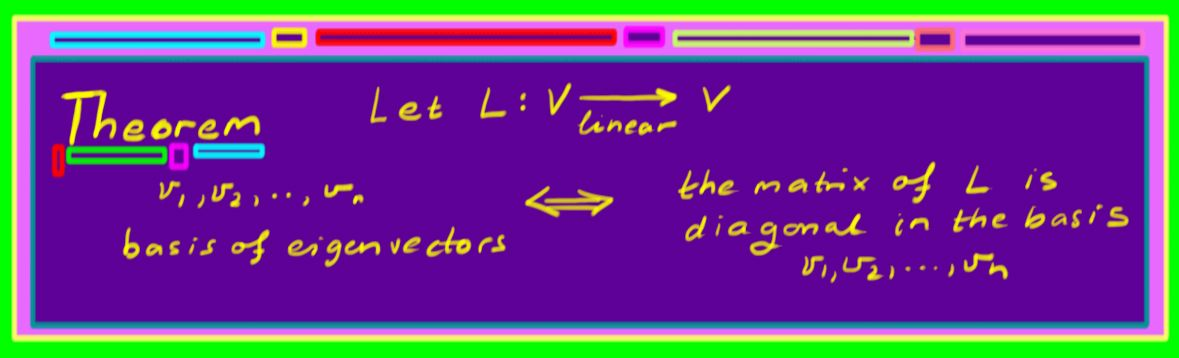
\includegraphics[scale=.33]{\diagPath/eigenbasis.jpg}
\end{center}
\caption{This theorem answers the question: ``What is diagonalization?''}
\end{figure}

%\section*{References}
%Hefferon, Chapter Three, Section V: Change of Basis
%\\
%Beezer, Chapter E, Section SD
%\\
%Beezer, Chapter R, Sections MR-CB
%\\
%Wikipedia:
%\begin{itemize}
%\item \href{http://en.wikipedia.org/wiki/Change_of_basis}{Change of Basis}
%\item \href{http://en.wikipedia.org/wiki/Diagonalizable_matrix}{Diagonalizable Matrix}
%\item \href{http://en.wikipedia.org/wiki/Similar_matrix}{Similar Matrix}
%\end{itemize}
%

\section{Review Problems}

{\bf Webwork:} 
\begin{tabular}{|c|c|}
\hline
Reading Problems & 
 \hwrref{Diagonalization}{1}, \hwrref{Diagonalization}{2}\\
No real eigenvalues &  \hwref{Diagonalization}{3}\\
Diagonalization &  \hwref{Diagonalization}{4}, \hwref{Diagonalization}{5},  \hwref{Diagonalization}{6},
 \hwref{Diagonalization}{7}\\
  \hline
\end{tabular}






\begin{enumerate}
\item \label{det33} Let $M=\begin{pmatrix}
m^1_1 & m^1_2 & m^1_3\\
m^2_1 & m^2_2 & m^2_3\\
m^3_1 & m^3_2 & m^3_3\\
\end{pmatrix}$.  Use row operations to put $M$ into \emph{row echelon form}.  For simplicity, assume that $m_1^1\neq 0 \neq m^1_1m^2_2-m^2_1m^1_2$.

Prove that $M$ is non-singular if and only if:
\[
m^1_1m^2_2m^3_3 
- m^1_1m^2_3m^3_2 
+ m^1_2m^2_3m^3_1 
- m^1_2m^2_1m^3_3 
+ m^1_3m^2_1m^3_2
- m^1_3m^2_2m^3_1
\neq 0
\]

\phantomnewpage

\item 
\begin{enumerate}
\item What does the matrix $E^1_2=\begin{pmatrix}
0 & 1 \\
1 & 0
\end{pmatrix}$ do to $M=\begin{pmatrix}
a & b \\
d & c
\end{pmatrix}$ under left multiplication?  What about right multiplication?
\item Find elementary matrices $R^1(\lambda)$ and $R^2(\lambda)$ that respectively multiply rows $1$ and $2$ of $M$ by $\lambda$ but otherwise leave $M$ the same under left multiplication.
\item Find a matrix $S^1_2(\lambda)$ that adds a multiple $\lambda$ of row $2$ to row $1$ under left multiplication.
\end{enumerate}

\phantomnewpage

\item Let $M$ be a matrix and $S^i_jM$ the same matrix with rows \(i\) and \(j\) switched.  Explain every line of the 
\hyperlink{rowswap}{series of equations} proving that $\det M = -\det (S^i_jM)$.

\phantomnewpage

%\item \label{prob_inversion_number} This problem is a ``hands-on'' look at why \hyperlink{permutation_parity}{the property} describing the parity of permutations is true.
%
%\hypertarget{inversion_number}{The \emph{inversion number}}\index{Permutation!Inversion number} of a permutation $\sigma$ is the number of pairs $i<j$ such that $\sigma(i)>\sigma(j)$; it's the number of ``numbers that appear left of smaller numbers'' in the permutation.  For example, for the permutation $\rho = [4,2,3,1]$, the inversion number is $5$. The number $4$ comes before $2,3,$ and $1$, and $2$ and $3$ both come before $1$.
%
%Given a permutation $\sigma$, we can make a new permutation $\tau_{i,j} \sigma$ by exchanging the $i$th and $j$th entries of $\sigma$.
%
%\begin{enumerate}
%\item What is the inversion number of the permutation \(\mu=[1,2,4,3]\) that exchanges 4 and 3 and leaves everything else alone? Is it an even or an odd permutation?
%
%\item What is the inversion number of the permutation \(\rho=[4,2,3,1]\) that exchanges 1 and 4 and leaves everything else alone? Is it an even or an odd permutation?
%
%\item What is the inversion number of the permutation \(\tau_{1,3} \mu\)? Compare the parity\footnote{The \emph{parity} of an integer refers to whether the integer is even or odd. Here the parity of a permutation $\mu$ refers to the parity of its inversion number.} of \(\mu\) to the parity of \(\tau_{1,3} \mu.\)
%
%\item What is the inversion number of the permutation \(\tau_{2,4} \rho\)? Compare the parity of \(\rho\) to the parity of \(\tau_{2,4} \rho.\)
%
%\item What is the inversion number of the permutation \(\tau_{3,4} \rho\)? Compare the parity of \(\rho\) to the parity of \(\tau_{3,4} \rho.\)
%\end{enumerate}
%
%\videoscriptlink{elementary_matrices_determinant_hint.mp4}{Problem~\ref{prob_inversion_number} hints}{scripts_elementary_matrices_determinants_hint}

\phantomnewpage

%\item \label{problem_permutation} (Extra credit) Here we will examine a (very) small set of the general properties about permutations and their applications. In particular, we will show that one way to compute the sign of a permutation is by finding the \hyperlink{inversion_number}{inversion number} $N$ of $\sigma$ and we have
%\[
%\sgn(\sigma) = (-1)^N.
%\]
%
%For this problem, let $\mu = [1,2,4,3]$.
%
%\begin{enumerate}
%\item Show that every permutation $\sigma$ can be sorted by only taking simple (adjacent) transpositions\index{Permutation!Simple transposition} $s_i$ where $s_i$ interchanges the numbers in position $i$ and $i+1$ of a permutation $\sigma$ (in our other notation $s_i = \tau_{i,i+1}$). For example $s_2 \mu = [1, 4, 2, 3]$, and to sort $\mu$ we have $s_3 \mu = [1, 2, 3, 4]$.
%
%\item \label{prob_part_relations} We can compose simple transpositions together to represent a permutation (note that the sequence of compositions is not unique), and these are associative, we have an identity (the trivial permutation where the list is in order or we do nothing on our list), and we have an inverse since it is clear that $s_i s_i \sigma = \sigma$. Thus permutations of $[n]$ under composition are an example of a \hyperref[groups]{group}. However note that not all simple transpositions commute with each other since
%\begin{align*}
%s_1 s_2 [1, 2, 3] & = s_1 [1, 3, 2] = [3, 1, 2]
%\\ s_2 s_1 [1, 2, 3] & = s_2 [2, 1, 3] = [2, 3, 1]
%\end{align*}
%(you will prove here when simple transpositions commute). When we consider our initial permutation to be the trivial permutation $e = [1, 2, \dotsc, n]$, we do not write it; for example $s_i \equiv s_i e$ and $\mu = s_3 \equiv s_3 e$. This is analogous to not writing 1 when multiplying. Show that $s_i s_i = e$ (in shorthand $s_i^2 = e$), $s_{i+1} s_i s_{i+1} = s_i s_{i+1} s_i$ for all $i$, and $s_i$ and $s_j$ commute for all $|i - j| \geq 2$.
%
%\item Show that every way of expressing $\sigma$ can be obtained from using the relations proved in part~\ref{prob_part_relations}. In other words, show that for any expression $w$ of simple transpositions representing the trivial permutation $e$, using the proved relations.
%
%\emph{Hint: Use induction on $n$. For the induction step, follow the path of the $(n+1)$-th strand by looking at $s_n s_{n-1} \cdots s_k s_{k\pm1} \cdots s_n$ and argue why you can write this as a subexpression for any expression of $e$. Consider using diagrams of these paths to help.}
%
%\item The simple transpositions \hyperlink{action}{acts on} an $n$-dimensional vector space $V$ by $s_i v = E^i_{i+1} v$ (where $E^i_j$ is \hyperlink{elem_matrix_row_swap}{an elementary matrix}) for all vectors $v \in V$. Therefore we can just represent a permutation $\sigma$ as the matrix $M_{\sigma}$\footnote{Often people will just use $\sigma$ for the matrix when the context is clear.}, and we have $\det(M_{s_i}) = \det(E^i_{i+1}) = -1$. Thus prove that $\det(M_{\sigma}) = (-1)^N$ where $N$ is a number of simple transpositions needed to represent $\sigma$ as a permutation. You can assume that $M_{s_i s_j} = M_{s_i} M_{s_j}$ (it is not hard to prove) and that $\det(A B) = \det(A) \det(B)$ \hyperref[detmultiplicative]{from Chapter~\ref*{elementarydeterminantsII}}.
%
%\emph{Hint: You to make sure $\det(M_{\sigma})$ is well-defined since there are infinite ways to represent $\sigma$ as simple transpositions.}
%
%\item Show that $s_{i+1} s_i s_{i+1} = \tau_{i, i+2}$, and so give one way of writing $\tau_{i, j}$ in terms of simple transpositions? Is $\tau_{i,j}$ an even or an odd permutation? What is $\det(M_{\tau_{i,j}})$? What is the inversion number of $\tau_{i,j}$?
%
%\item The minimal number of simple transpositions needed to express $\sigma$ is called the \emph{length}\index{Permutation!Length} of $\sigma$; for example the length of $\mu$ is 1 since $\mu = s_3$. Show that the length of $\sigma$ is equal to the inversion number of $\sigma$.
%
%\emph{Hint: Find an procedure which gives you a new permutation $\sigma^{\prime}$ where $\sigma = s_i \sigma^{\prime}$ for some $i$ and the inversion number for $\sigma^{\prime}$ is 1 less than the inversion number for $\sigma$.}
%
%\item Show that $(-1)^N = \sgn(\sigma) = \det(M_{\sigma})$, where $\sigma$ is a permutation with $N$ inversions. Note that this immediately implies that $\sgn(\sigma \rho) = \sgn(\sigma) \sgn(\rho)$ for any permutations $\sigma$ and $\rho$.
%\end{enumerate}

\item Let $M'$ be the matrix obtained from $M$ by swapping two columns $i$ and $j$. Show that $\det M'=-\det M $.

\item The scalar triple product of three vectors $u,v,w$ from $\Re^3$ is $u\cdot(v\times w)$. Show that this product is the same as the determinant of the matrix whose columns are $u,v,w$ (in that order). What happens to the scalar triple product when the factors are permuted? 

\item Show that if $M$ is a $3\times 3$ matrix whose third row is a sum of multiples of the other rows ($R_3=aR_2+bR_1$) then $\det M=0$. Show that the same is true if one of the columns is a sum of multiples of the others. 

\end{enumerate}

\phantomnewpage

\newpage

